\documentclass[12pt]{article}
\usepackage{amsmath}
\usepackage{amssymb}
\usepackage{amsthm}
\usepackage{setspace}
\usepackage{fancyhdr}
\usepackage{color}
\usepackage{subcaption}
\usepackage{xfrac}
\usepackage{graphicx}
\usepackage{cite} %if auctex does not prompt bibtex use "C-c C-n"
\usepackage[margin=.75in]{geometry} %Sets margin size
\newcommand{\vp}{\varphi}
\newcommand{\dif}{\text{d}}
\pagestyle{fancy}
\begin{document}
%\lhead{APMA 990}
%\rhead{Final Project}
\title{A Comparative Study of the TV and Ginzburg--Landau Inpainting Models}
\date{\today}
\author{Ray Walsh\\
301257297}
% \maketitle
% \doublespacing

\begin{figure}[tb!]
  \centering
  \begin{subfigure}{.5\linewidth}
    \centering
    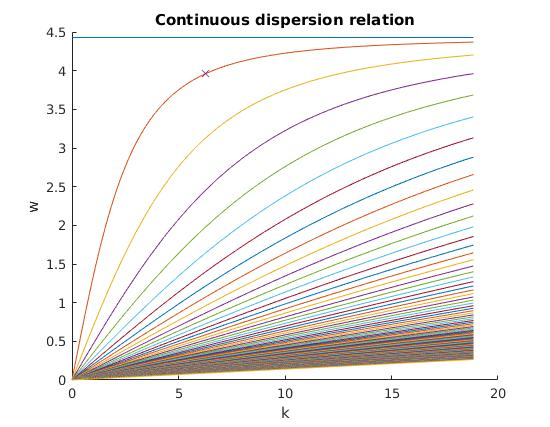
\includegraphics[width=\linewidth]{CDRel.jpg}
    \caption{}
    \label{fig:WideCross}
  \end{subfigure}%
  \begin{subfigure}{.5\linewidth}
    \centering
    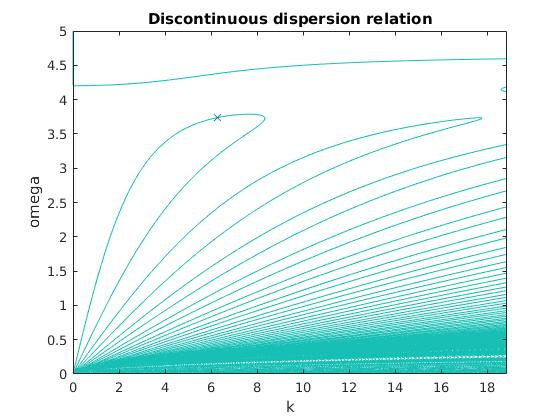
\includegraphics[width=\linewidth]{DDRel.jpg}
    \caption{}
    \label{fig:InpaintedWideCross}
  \end{subfigure}\\[1ex]
  \caption{Results of the TV inpainting model for the ambiguous entangled man. Notice how the TV model also prefers the interpretation of the mans torso in front of the fence.}
  \label{fig:TVWideCross}
\end{figure}
\end{document}





%%% Local Variables: 
%%% mode: latex
%%% TeX-master: t
%%% End: 
